\documentclass[11pt,a4paper]{article}

% ---------- Packages ----------
\usepackage[T1]{fontenc}
\usepackage[utf8]{inputenc}
\usepackage{lmodern}
\usepackage{microtype}
\usepackage[margin=2.5cm]{geometry}
\usepackage{graphicx}
\usepackage{booktabs}
\usepackage{tabularx}
\usepackage{array}
\usepackage[table]{xcolor}
\usepackage{amsmath}
\usepackage{siunitx}
\usepackage{caption}
\usepackage[numbers,sort&compress]{natbib}
\usepackage{url}
\usepackage[hidelinks]{hyperref}

\captionsetup{font=small,labelfont=bf}
\definecolor{best}{RGB}{226,239,218}
\newcommand{\best}[1]{\cellcolor{best}\textbf{#1}}
\newcolumntype{L}{>{\raggedright\arraybackslash}X}

\title{Comparing Multi-Object Tracking Algorithms for\\Stable Real-Time YOLOv8 Tracking}
\author{Jerome Loke\\
\small\texttt{lokejer@gmail.com}}
\date{2026}

\begin{document}
\maketitle

% ---------- Abstract ----------
\begin{abstract}
Stable pedestrian tracking requires more than detecting people independently in each video frame. A real-time system must maintain identities through motion, occlusion and missed detections without introducing excessive computational latency. This study presents a controlled comparison of five multi-object tracking algorithms, ByteTrack, BoT-SORT, TrackTrack, Deep OC-SORT with ReID, and FastTracker, paired with the same YOLOv8l detector and evaluated on the MOT17-09 pedestrian sequence. Detector configuration, preprocessing, input frames and evaluation procedure were held constant so that differences could be attributed primarily to the tracking configurations. Tracking performance was evaluated using HOTA, AssA, IDF1, MOTA, identity switches and fragmentation, while deployment performance was measured using median latency, P95 latency and throughput. TrackTrack achieved the strongest overall quality, with 48.17\% HOTA and 58.08\% IDF1, but processed only 18.51~FPS. In contrast, ByteTrack achieved the highest throughput at 38.81~FPS with a median latency of 25.26~ms, while retaining 44.48\% HOTA. Under the tested laptop configuration, ByteTrack therefore provides the most practical quality-speed balance for real-time deployment, whereas TrackTrack is preferable when tracking quality is prioritised over frame rate.
\end{abstract}

\noindent\textbf{Code and data:} \url{https://github.com/lokejer/MOT-algo-benchmark}

% ---------- 1 Introduction ----------
\section{Introduction}

Real-time video analytics often begins with an object detector such as YOLO, which locates people independently within each frame. Detection alone, however, does not determine whether a person observed in one frame is the same person observed later. \textbf{Multi-object tracking (MOT)} adds this temporal association layer by assigning persistent identities across frames. Maintaining these identities becomes difficult when pedestrians overlap, become temporarily occluded, change direction, or are missed by the detector. Modern tracking-by-detection methods therefore differ substantially in how they associate current detections with existing trajectories~\cite{bewley2016sort,wojke2017deepsort,zhang2022bytetrack,cao2023ocsort,aharon2022botsort}.

For an operational real-time system, tracking quality is only one requirement. More sophisticated association strategies can use additional motion history, appearance information or recovery mechanisms to preserve identities, but these operations may increase processing latency. Real-time MOT research has similarly recognised that computational efficiency must be considered alongside tracking accuracy rather than treating association speed separately. A tracker that improves identity consistency but processes substantially below the \textbf{30~FPS input rate} may therefore be less suitable for live laptop deployment.

This study addresses the research question: \emph{How do different multi-object tracking algorithms compare in tracking stability and real-time performance when paired with the same YOLOv8 object detector?} Five modern trackers are evaluated: ByteTrack, BoT-SORT, TrackTrack, Deep OC-SORT with ReID, and FastTracker. Tracking stability is assessed using \textbf{HOTA} and \textbf{AssA} for overall and association quality, \textbf{IDF1} for identity preservation, and \textbf{identity switches and fragmentation} for direct tracking failures. Real-time performance is assessed using median and P95 latency together with throughput in frames per second. This combination is important because MOT methods can produce different accuracy-speed trade-offs even when used with the same detector.

To isolate these differences, the experiment holds the \textbf{YOLOv8l detector, person-only class filter, 0.10 confidence threshold, 640-pixel inference size, preprocessing, MOT17-09 input frames and evaluation procedure constant}. Only the tracker configuration changes between runs. The contribution is therefore not a new tracking algorithm, but a \textbf{controlled and reproducible implementation comparison} that examines how different association strategies affect identity stability and laptop runtime under the same detection pipeline. The resulting comparison provides a deployment-oriented recommendation for selecting between higher tracking quality and real-time throughput.

% ---------- 2 Related Work ----------
\section{Related Work}

\subsection{Tracking-by-detection baseline and appearance association}

\paragraph{SORT.} Simple Online and Realtime Tracking (SORT) provides a lightweight tracking-by-detection baseline. It uses a \textbf{Kalman filter} to predict each tracked object's position in the next frame, then applies the \textbf{Hungarian algorithm} to match new detections with predicted tracks based on bounding-box overlap. This simple design enables fast online tracking, but association relies primarily on motion and spatial information. Consequently, identities can be difficult to recover when objects are occluded for longer periods or leave and re-enter the scene, increasing the risk of identity switches~\cite{bewley2016sort}.

\paragraph{DeepSORT.} DeepSORT extends SORT by incorporating a learned \textbf{appearance descriptor}, or person re-identification (ReID) feature, into data association. Instead of relying only on motion, detections can also be matched to tracks according to visual similarity. This allows the tracker to better preserve identities through occlusion and reduces identity switches. The original study reported a \textbf{45\% reduction in identity switches} over SORT. However, extracting and comparing appearance embeddings introduces additional computation compared with SORT's simpler motion-based association~\cite{wojke2017deepsort}.

These methods establish an important trade-off for this study: \textbf{motion-only association prioritises efficiency, while appearance-assisted association can improve identity consistency at additional computational cost}. This distinction motivates evaluating both tracking quality and runtime when comparing more advanced MOT algorithms.

\subsection{Modern association strategies}

\paragraph{ByteTrack.} ByteTrack performs a second association stage using lower-confidence detections that may still correspond to partially occluded objects. Recovering these detections can reduce broken trajectories while retaining a relatively lightweight association process~\cite{zhang2022bytetrack}.

\paragraph{OC-SORT.} OC-SORT addresses motion-prediction drift during occlusion by using observed detections to correct accumulated Kalman-filter errors. Its observation-centric design improves robustness to occlusion and non-linear motion while remaining primarily motion-based~\cite{cao2023ocsort}.

\paragraph{BoT-SORT.} BoT-SORT combines motion association, camera-motion compensation and optional appearance/ReID cues~\cite{aharon2022botsort}. These additional components can strengthen association but increase computational complexity. In this experiment, ReID is disabled, so the tested configuration does not represent the complete ReID-enabled BoT-SORT pipeline.

\paragraph{TrackTrack.} TrackTrack introduces Track-Perspective-Based Association, which selects detections from the perspective of existing tracks, together with Track-Aware Initialization to reduce unnecessary new identities~\cite{shim2025tracktrack}. These mechanisms are designed to preserve established trajectories and reduce identity switches and fragmentation, although the additional association logic may increase runtime.

\paragraph{Deep OC-SORT + ReID.} Deep OC-SORT extends OC-SORT by adaptively incorporating appearance-based ReID features into motion association~\cite{maggiolino2023deepocsort}. Appearance cues can help recover identities when motion becomes ambiguous during occlusion, but feature extraction introduces additional computation.

\paragraph{FastTracker.} FastTracker uses a lightweight ByteTrack-based association approach with additional occlusion-aware track retention~\cite{hashempoor2025fasttracker}. This aims to preserve lost tracks during temporary occlusion without the heavier appearance-processing cost of ReID-based methods, making it relevant to real-time tracking~\cite{ultralytics_track}.

Together, these approaches represent different quality-speed trade-offs: ByteTrack and FastTracker emphasise efficient association, TrackTrack strengthens trajectory preservation, Deep OC-SORT adds adaptive appearance matching, while BoT-SORT combines multiple motion-related cues. These differences form the basis for the controlled comparison in this study.

\subsection{Comparison gap}

The original tracker papers demonstrate strong results, but their reported performance is obtained under different detectors, datasets, configurations and hardware. Directly comparing their published benchmark values therefore does not isolate the effect of the association strategy itself. This study instead asks a narrower practical question: when the detector, input sequence and evaluation pipeline are held constant on the same laptop, which association strategy provides the most useful balance between identity stability and real-time speed? This controlled design allows differences in metrics such as IDF1, ID switches, fragmentation and FPS to be interpreted more directly as differences between tracker configurations.

% ---------- 3 Method ----------
\section{Dataset, System and Methodology}

\subsection{Fixed detection pipeline and tracker variants}

All five experiments use the same pre-trained YOLOv8l detector with a person-only class filter and a detection confidence threshold of 0.10. This threshold is intentionally chosen to allow more candidate detections to be passed to the tracking algorithm. This is especially relevant for methods such as ByteTrack which use lower-confidence detections to recover difficult or partially occluded objects.

Each tracker is evaluated from a fresh YOLO model and tracker state to prevent information from one run carrying into another. Every algorithm processes the same MOTChallenge sequence, with predictions recorded frame-by-frame as bounding boxes, confidence scores, class IDs and track IDs. The exact repository version, tracker configuration files and software package versions are recorded to support reproducibility.

Finally, tracking performance is evaluated using a suite of complementary metrics rather than relying on a single score. \textbf{HOTA} is used as the main overall tracking metric because it balances detection accuracy and association accuracy, while \textbf{IDF1} measures how consistently object identities are maintained across frames. Additional metrics include MOTA, DetA, AssA, ID switches, track fragments, precision, and recall~\cite{luiten2021hota}. Runtime is evaluated using median latency, P95 latency, and throughput in frames per second. Table~\ref{tab:trackers} summarises the tracker variants.

\begin{table}[!htbp]
\centering
\small
\caption{Tracker variants evaluated under the same YOLOv8 detection pipeline.}
\label{tab:trackers}
\begin{tabularx}{\linewidth}{@{}l L L@{}}
\toprule
\textbf{Tracker} & \textbf{Main association idea} & \textbf{Expected strength} \\
\midrule
ByteTrack & Two-stage association using high- and low-confidence detections & Fast tracking with recovery of partially occluded detections \\
BoT-SORT & Motion association with camera-motion compensation; ReID disabled in this experiment & Stronger association than basic motion-only tracking \\
TrackTrack & Track-perspective association and track-aware initialisation & Strong identity stability and fewer ID switches/fragments \\
Deep OC-SORT + ReID & Observation-centric motion with adaptive appearance/ReID matching & Better identity recovery during occlusion and ambiguous motion \\
FastTracker & Lightweight ByteTrack-based association with occlusion-aware track retention & Good real-time speed with improved track continuity \\
\bottomrule
\end{tabularx}
\end{table}

\subsection{Evaluation dataset and preprocessing}

The experiment uses the \textbf{MOT17-09 pedestrian-tracking sequence}, consisting of \textbf{525 frames at 1920$\times$1080 and 30~FPS}, with \textbf{5,325 pedestrian annotations across 26 ground-truth trajectories}~\cite{dendorfer2021motchallenge}. The same video frames and annotations are used for all five trackers, ensuring that differences in performance are not caused by different input data. Figure~\ref{fig:frame} shows an example frame with its ground truth, and Figure~\ref{fig:challenges} illustrates conditions that make the sequence challenging.

\begin{figure}[!htbp]
\centering
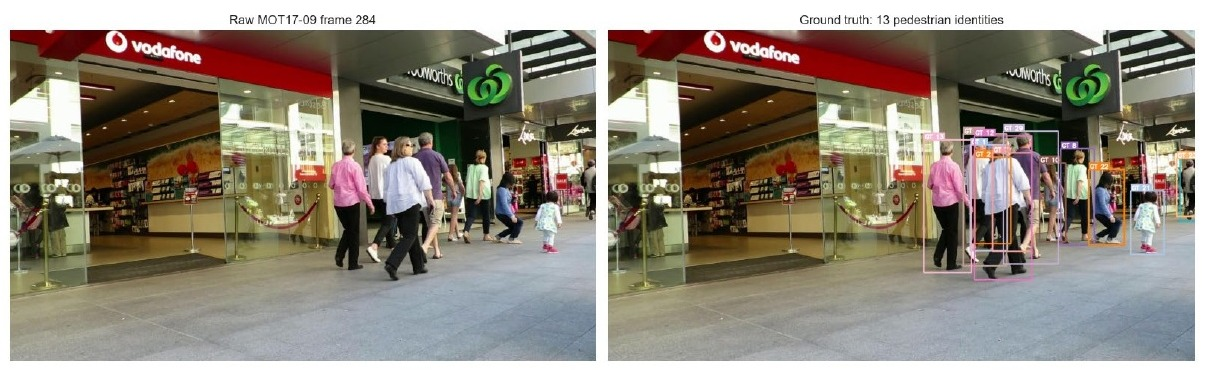
\includegraphics[width=\linewidth]{figures/mot17_frame_gt.jpg}
\caption{Example frame of the MOT17-09 person-tracking sequence (left) and its ground-truth annotations (right).}
\label{fig:frame}
\end{figure}

\begin{figure}[!htbp]
\centering
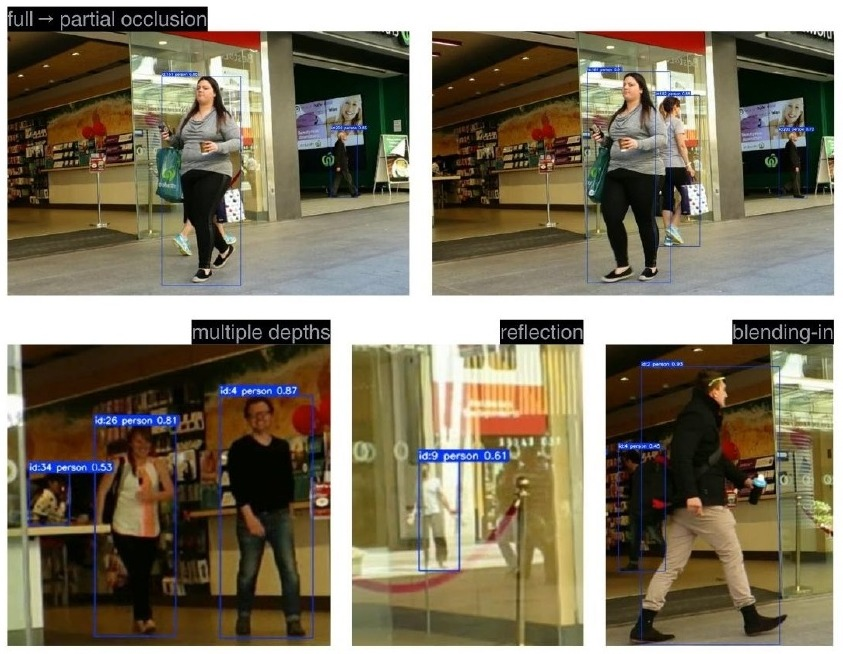
\includegraphics[width=0.62\linewidth]{figures/challenging_conditions.jpg}
\caption{Examples of challenging pedestrian-tracking conditions in MOT17-09: full-to-partial occlusion, multiple depths, reflections, and pedestrians blending into the background.}
\label{fig:challenges}
\end{figure}

Ground-truth annotations are loaded in MOTChallenge format using the frame number, identity and bounding-box coordinates $(x, y, \text{width}, \text{height})$. Tracker predictions are recorded in the same bounding-box representation together with their assigned track IDs. For identity and CLEAR MOT evaluation, predicted and ground-truth boxes are matched using \textbf{Intersection over Union (IoU)} with a threshold of \textbf{0.50}.

The local evaluator does not reproduce the full official MOTChallenge treatment of \textbf{distractors and ignore regions}. Therefore, the reported scores should not be interpreted as official MOTChallenge benchmark results. However, because every tracker is evaluated using the \textbf{same sequence, ground truth and matching procedure}, the results remain suitable for the controlled relative comparison required in this study.

\subsection{Evaluation metrics}

Table~\ref{tab:metrics} maps each evaluation question to the metrics used to answer it.

\begin{table}[!htbp]
\centering
\small
\caption{Metrics used to evaluate tracking stability and deployment performance.}
\label{tab:metrics}
\begin{tabularx}{\linewidth}{@{}l l L@{}}
\toprule
\textbf{Question} & \textbf{Primary metrics} & \textbf{Interpretation} \\
\midrule
Overall tracking quality & HOTA & Balances detection and association quality \\
Identity stability & IDF1, AssA, ID switches, fragments & Measures whether identities stay consistent over time \\
Detection contribution & DetA, precision, recall & Separates detector-related misses/false positives from association quality \\
Real-time performance & Median latency, P95 latency, FPS & Shows typical speed, worst-case tendency and live-video viability \\
\bottomrule
\end{tabularx}
\end{table}

\subsection{Experimental protocol and reproducibility}

To improve timing reliability, GPU synchronisation is performed immediately before and after each timed inference, and the first five frames are excluded as warm-up frames. Runtime measurement begins before frame capture and ends after the tracking results are returned and transferred for collection. Rendering and MP4 encoding are performed outside the timer, so the reported latency reflects capture, preprocessing, detection and tracking rather than display overhead.

For reproducibility, the notebook records the Git commit, Python, PyTorch, CUDA, Ultralytics, OpenCV, NumPy, pandas, SciPy and Matplotlib versions, together with the processing device and GPU. It also resolves and records the exact tracker configuration files used. Each run saves frame-level predictions to CSV, annotated videos, and the final aggregate comparison table. Assertions verify that all five trackers complete the expected 525 frames, produce valid prediction schemas, and return finite positive timing results. All experiments were run on an NVIDIA GeForce RTX 5060 Laptop GPU.

% ---------- 4 Results ----------
\section{Results}

\subsection{Overall comparison}

Table~\ref{tab:results} reports the main tracking-quality and runtime results; the best value in each column is highlighted. Figure~\ref{fig:tradeoff} plots HOTA against throughput.

\begin{table}[!htbp]
\centering
\footnotesize
\setlength{\tabcolsep}{2pt}
\caption{Main tracking-quality and runtime comparison (best value per column highlighted). $\uparrow$: higher is better; $\downarrow$: lower is better.}
\label{tab:results}
\begin{tabular}{@{}l *{10}{c}@{}}
\toprule
\textbf{Tracker} & \textbf{HOTA}$\uparrow$ & \textbf{IDF1}$\uparrow$ & \textbf{AssA}$\uparrow$ & \textbf{IDSw}$\downarrow$ & \textbf{Frag}$\downarrow$ & \textbf{Prec.}$\uparrow$ & \textbf{Rec.}$\uparrow$ & \textbf{\shortstack{Med.\\lat. (ms)}}$\downarrow$ & \textbf{\shortstack{P95\\lat. (ms)}}$\downarrow$ & \textbf{FPS}$\uparrow$ \\
\midrule
ByteTrack       & 44.48 & 50.69 & 40.70 & 43 & 61 & 75.14 & 71.57 & \best{25.26} & \best{29.35} & \best{38.81} \\
BoT-SORT        & 46.36 & 54.05 & 42.70 & 45 & 57 & 76.37 & \best{73.01} & 53.18 & 58.96 & 18.76 \\
TrackTrack      & \best{48.17} & \best{58.08} & \best{44.30} & \best{29} & \best{49} & \best{85.84} & 68.86 & 53.69 & 59.26 & 18.51 \\
Deep OC-SORT+ReID & 44.66 & 52.87 & 40.79 & 47 & 62 & 76.41 & 71.77 & 29.12 & 34.30 & 33.63 \\
FastTracker     & 44.15 & 51.78 & 40.51 & 56 & 59 & 75.32 & 71.81 & 27.54 & 31.12 & 35.76 \\
\bottomrule
\end{tabular}

\end{table}

\begin{figure}[!htbp]
\centering
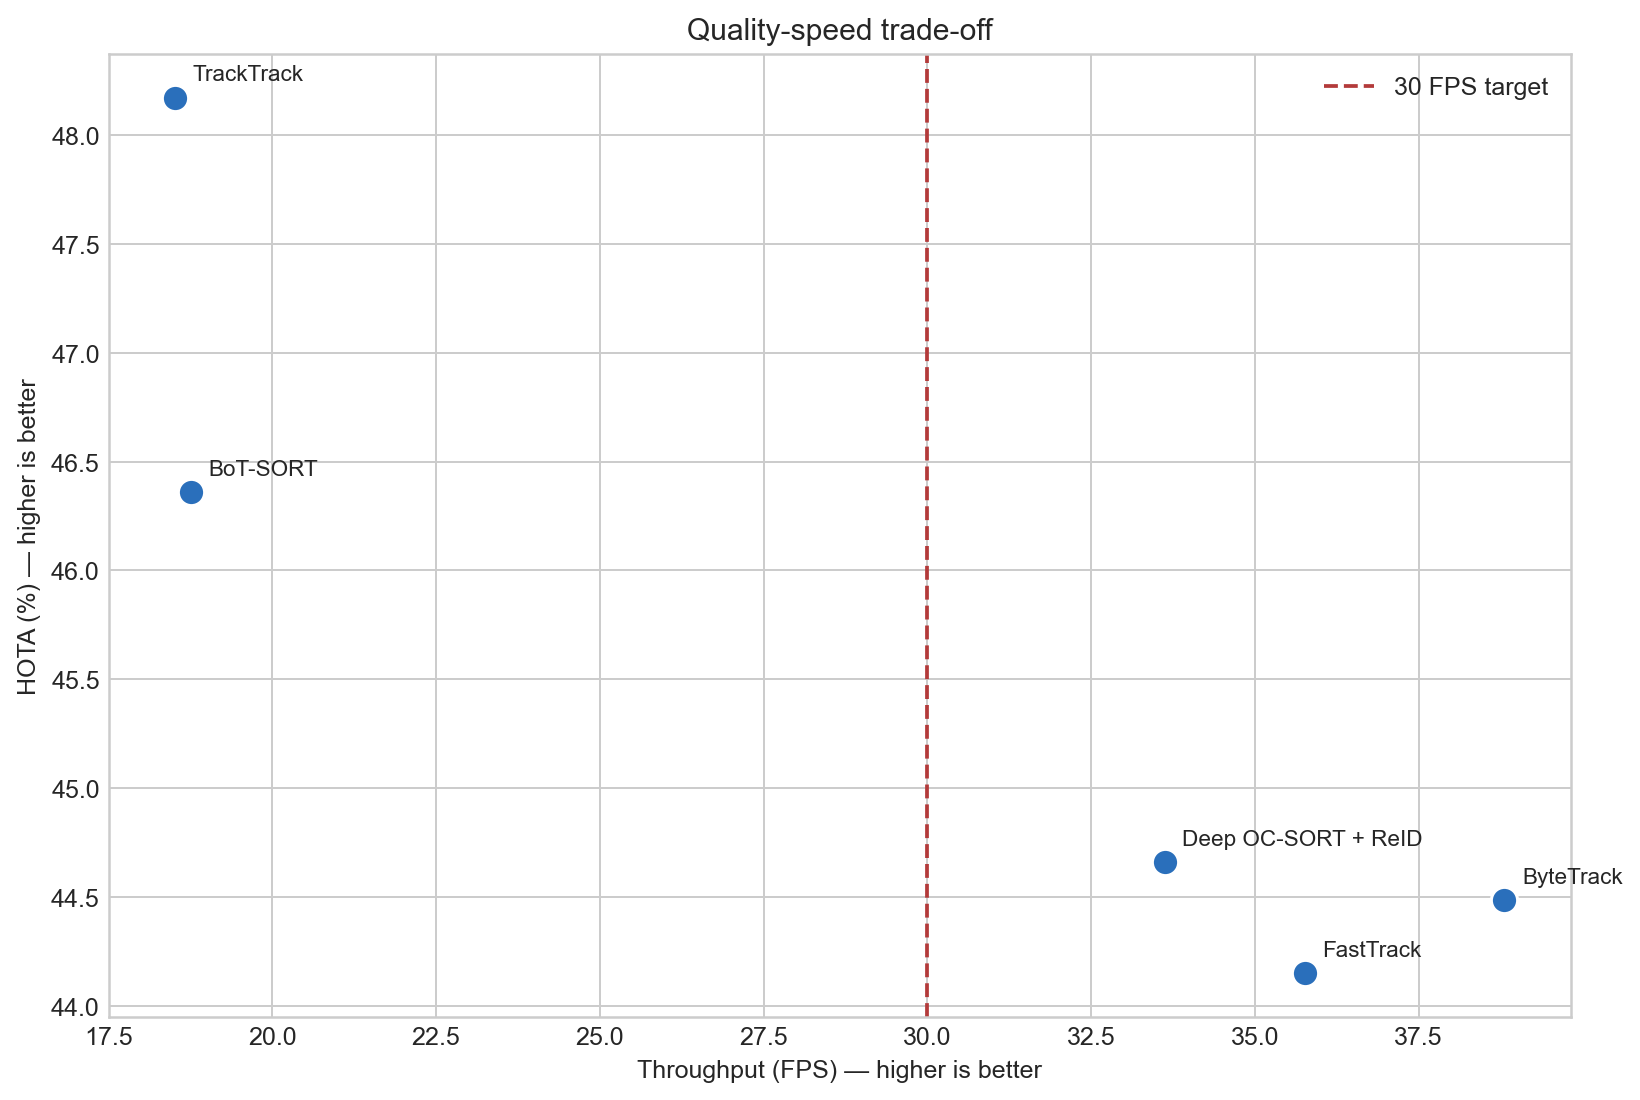
\includegraphics[width=0.75\linewidth]{figures/quality_speed_tradeoff.png}
\caption{Quality-speed trade-off between HOTA and throughput for the five trackers. The dashed line marks the 30~FPS real-time target.}
\label{fig:tradeoff}
\end{figure}

\begin{figure}[!htbp]
\centering
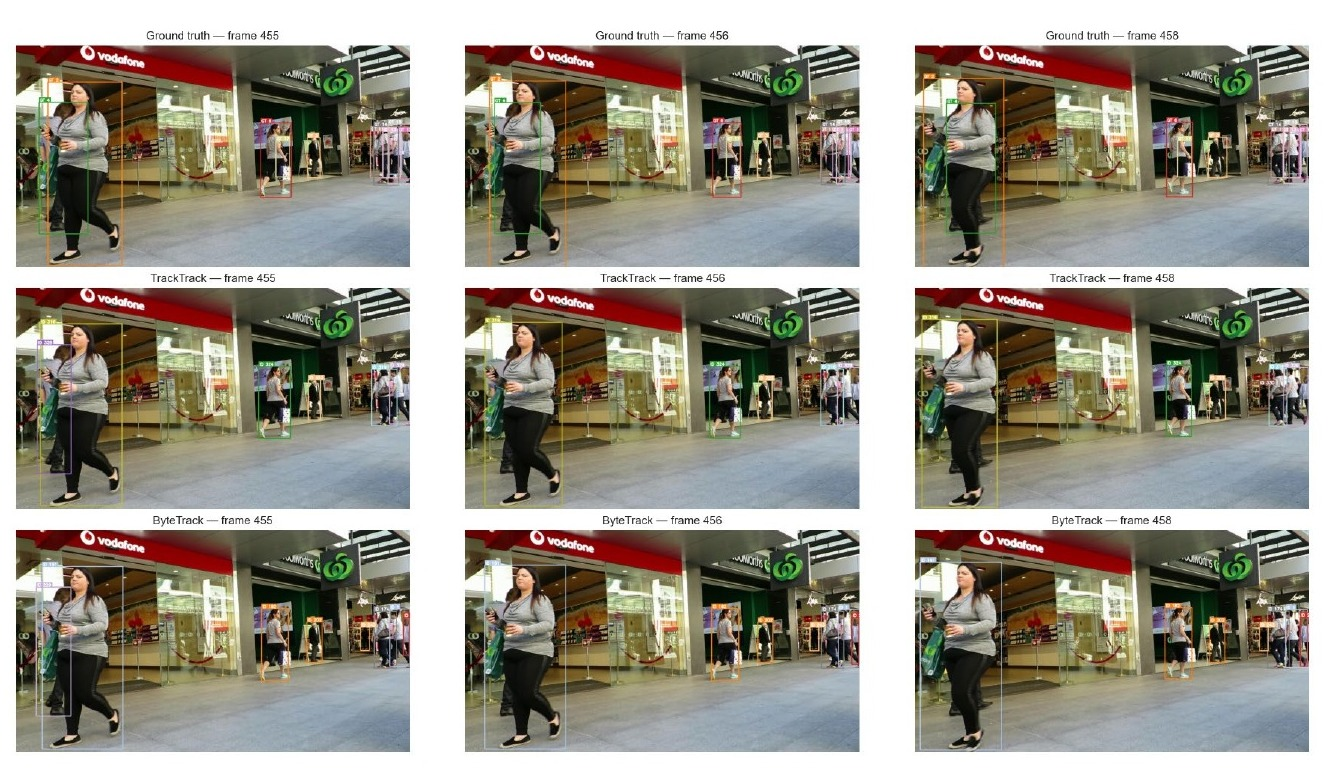
\includegraphics[width=\linewidth]{figures/qualitative_tracktrack_bytetrack.jpg}
\caption{Qualitative comparison of ground truth (top), TrackTrack, the highest-quality tracker (middle), and ByteTrack, the fastest tracker (bottom), across frames 455--458 of a challenging pedestrian sequence.}
\label{fig:qualitative}
\end{figure}

\subsection{Result interpretation}

This section identifies (1) best overall quality, (2) best identity stability, (3) fastest tracker, and (4) best quality-speed compromise.

\paragraph{Best overall quality.} TrackTrack achieved the \textbf{best overall tracking quality}, recording the highest HOTA at 48.17\%, 1.81 percentage points above BoT-SORT at 46.36\%. It also achieved the highest DetA (52.55\%), AssA (44.30\%), and MOTA (56.96\%). This is consistent with its track-focused association design, where Track-Perspective-Based Association selects detections from the perspective of existing tracks and Track-Aware Initialization suppresses unnecessary new tracks~\cite{shim2025tracktrack}. Its advantage came at a substantial runtime cost, however, reaching only 18.51~FPS with a median latency of 53.69~ms.

\paragraph{Best identity stability.} TrackTrack also provided the \textbf{strongest identity stability}. It achieved the highest IDF1 at 58.08\%, 4.03 percentage points above BoT-SORT, while producing only 29 identity switches and 49 fragments, the lowest values among all five trackers. This result is consistent with TrackTrack's explicit aim of preserving existing trajectories and suppressing spurious track initiation~\cite{shim2025tracktrack}. Surprisingly, Deep OC-SORT + ReID did not outperform TrackTrack in identity stability, despite adaptively incorporating appearance information into the motion-based OC-SORT framework~\cite{maggiolino2023deepocsort}. It achieved 52.87\% IDF1 and 47 identity switches. On this short sequence, TrackTrack's track-focused association appears to have been more effective than the additional ReID cue, although this result should not be generalised beyond the tested sequence.

\paragraph{Fastest tracker.} ByteTrack was the \textbf{fastest tracker}, achieving 38.81~FPS and the lowest median latency of 25.26~ms. It was 3.05~FPS faster than the next-fastest FastTracker and more than twice as fast as TrackTrack. This is consistent with ByteTrack's relatively simple association strategy, which recovers objects from lower-confidence detection boxes by associating them with existing tracklets, without requiring an appearance/ReID model~\cite{zhang2022bytetrack}. Its quality was lower, however, with 44.48\% HOTA and 50.69\% IDF1. The result demonstrates the expected speed-quality trade-off rather than one tracker dominating every metric.

\paragraph{Best quality-speed compromise.} For the \textbf{best quality-speed compromise}, ByteTrack is selected by the experiment's equal-weight harmonic mean of relative HOTA and FPS. Although its HOTA was 3.69 percentage points below TrackTrack, it delivered 20.30 additional FPS and exceeded the 30~FPS real-time target. Deep OC-SORT + ReID also produced a notable compromise at 33.63~FPS and a higher IDF1 of 52.87\%, showing that adaptive appearance-assisted association~\cite{maggiolino2023deepocsort} did not necessarily prevent real-time operation in this experiment. Overall, TrackTrack is preferable when tracking and identity quality are prioritised, while ByteTrack provides the strongest balance when real-time laptop deployment is also required.

% ---------- 5 Discussion ----------
\section{Discussion}

For a \textbf{30~FPS laptop-based live system, ByteTrack is the preferred choice}. It achieved the highest throughput at \textbf{38.81~FPS} with a median latency of \textbf{25.26~ms}, while maintaining 44.48\% HOTA. In contrast, \textbf{TrackTrack is better suited to offline or quality-focused processing}, achieving the highest HOTA (\textbf{48.17\%}) and IDF1 (\textbf{58.08\%}), but only \textbf{18.51~FPS}. The results therefore show that the highest tracking quality does not necessarily provide the most practical real-time deployment.

The observed differences are broadly consistent with the trackers' association designs. ByteTrack's relatively lightweight strategy associates lower-confidence detections to recover missed objects without an appearance model~\cite{zhang2022bytetrack}, which is consistent with its strong runtime. TrackTrack's track-focused association and suppression of unnecessary track initialisation~\cite{shim2025tracktrack} correspond with its lowest \textbf{29 identity switches} and \textbf{49 fragments}. Deep OC-SORT uses adaptive ReID to supplement motion-based association~\cite{maggiolino2023deepocsort}, achieving a stronger IDF1 of \textbf{52.87\%} than ByteTrack while still reaching \textbf{33.63~FPS}. BoT-SORT's richer motion and association pipeline~\cite{aharon2022botsort} achieved higher HOTA than ByteTrack, but at substantially lower throughput.

From a deployment perspective, MOT systems should therefore be selected according to both tracking quality and hardware constraints. Occlusion, camera motion and scene density may increase the value of stronger association methods, while latency becomes critical for live applications. These conclusions are limited to \textbf{MOT17-09, pedestrian tracking, YOLOv8l and the tested laptop hardware}. In addition, the local evaluator does not reproduce the full official MOTChallenge handling of distractors and ignore regions, and differences between third-party tracker implementations may affect results. Each tracker was also timed in a single run, so runtime variance is not characterised. The findings should therefore be interpreted as a \textbf{controlled relative comparison}, rather than official benchmark performance.

% ---------- 6 Conclusion ----------
\section{Conclusion}

This study compared five multi-object tracking configurations under the same YOLOv8l detection pipeline to determine how association strategy affects tracking stability and real-time performance. Keeping the detector, input sequence and evaluation procedure constant enabled a direct comparison of the trackers under the tested laptop environment.

\textbf{TrackTrack achieved the strongest overall tracking quality}, recording the highest HOTA of \textbf{48.17\%} and IDF1 of \textbf{58.08\%}, together with the fewest identity switches and fragments. However, its throughput of \textbf{18.51~FPS} fell below the 30~FPS requirement for live processing. In contrast, \textbf{ByteTrack was the fastest tracker}, reaching \textbf{38.81~FPS} with a median latency of \textbf{25.26~ms}, while maintaining 44.48\% HOTA. For the tested real-time laptop application, ByteTrack therefore provides the most practical quality-speed balance, while TrackTrack is better suited when tracking quality is prioritised over processing speed.

The main limitation is that evaluation was restricted to the \textbf{MOT17-09 pedestrian sequence} using a local evaluator rather than the complete official MOTChallenge protocol.

\section{Future Work}

The most important next step is evaluation across additional MOT17 sequences with different density, motion, lighting, and camera movement, followed by official ignore-region handling and repeated timing trials.

\bibliographystyle{unsrtnat}
\bibliography{refs}

\end{document}
